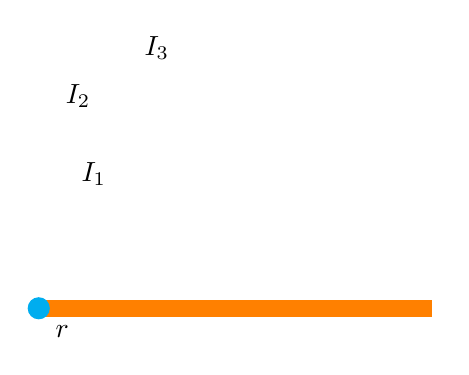
\begin{tikzpicture}

\creategrid{6}{4}
\drawobstacle{0}{3}
\drawobstacle{1}{3}
\drawobstacle{0}{0}
\drawobstacle{3}{1}
\drawobstacle{4}{1}

\coordinate (r) at (1,0);
\coordinate (rp) at (3,2);
\coordinate (i) at (2,2);
\coordinate (ip1) at (3,3);
\coordinate (ip2) at (5,2);
\coordinate (ip3) at (5,3);

%\path[name path=p1] (1,0) -- +(4,4);
%\path[name path=p2] (0,3) -- (6,3);
%\path[name path=p3] (0,2) -- (6,2);

%\draw[name intersections={of=p1 and p3,by=x2}];
%\draw[orange,line width=6] (1,2) -- (x2);
%\draw[orange,line width=6] (1,2) -- (x2);
\draw[orange,line width=6] (1,0) -- (6,0);
%\draw[cyan, line width=6] (x2) -- +(2,0);

%\draw[name intersections={of=p1 and p2,by=x1}];
%\draw[orange,line width=6] (1,3) -- (x1);
%\draw[cyan, line width=6] (x1) -- (6,3);

%\draw[black, dashed, line width=2] (1,0) -- (1,3);
%\draw[black, dashed, line width=2] (1,0) -- (x2);
%\draw[black, dashed, line width=2] (1,0) -- (x1);
%\draw[black, dashed, line width=1] (1,0) -- (2,3);

%\fill[orange] (3,3) circle(4pt);
\fill[cyan] (1,0) circle(4pt);

\draw (r) +(0.3, -0.3) node {$r$} + (0, 0) -- (r);
%\draw (rp) +(-0.15, -0.35) node {$r'$} + (0, 0) -- (rp);
\draw (i) +(-0.3, -0.3) node {$I_1$} + (0, 0) -- (i);
\draw (ip1) +(-1.5, -0.3) node {$I_2$} + (0, 0) -- (ip1);
\draw (ip1) +(-0.5, 0.3) node {$I_3$} + (0, 0) -- (ip1);
%\draw (ip2) +(-0.5, 0.3) node {$I'_3$} + (0, 0) -- (ip2);
%\draw (ip3) +(-0.5, 0.3) node {$I'_4$} + (0, 0) -- (ip3);
%\draw (i) +(-0.5, 0.5) node {I} + (0, 0) -- (i);

\end{tikzpicture}
